\section{Choosing Q(z)}
\begin{frame}
    \frametitle{Outline}
    \tableofcontents[currentsection]
\end{frame}

\begin{frame}
    \frametitle{Choosing $Q(z)$}
    Closed-loop dynamics:
    \alignbox{
        P = \frac{G_n(1+\Delta)(1-Q)}{1+Q \Delta} D + \frac{G_n(1+\Delta)}{1+Q \Delta} \bar{U}
            - \frac{Q(1+\Delta)}{1+Q \Delta} V
    }

    Concerns when choosing $Q(z)$:
    \begin{enumerate}
    \item \textbf{Robust disturbance rejection:}
    Choose $Q(e^{j\omega}) \approx 1$ at frequencies for which disturbance rejection is important
    \pause

    \item \textbf{Sensor noise insensitivity:}
    Choose $|Q(e^{j\omega})|$ to be small at frequencies for which sensor noise is large
    \pause

    \item \textbf{Robustness:}
    Choose $|Q(e^{j\omega})|$ to be small at frequencies for which $|\Delta(e^{j\omega})|$ is large
    \end{enumerate}
\end{frame}

\begin{frame}
    \frametitle{Choosing $Q(z)$}

    \begin{figure}
        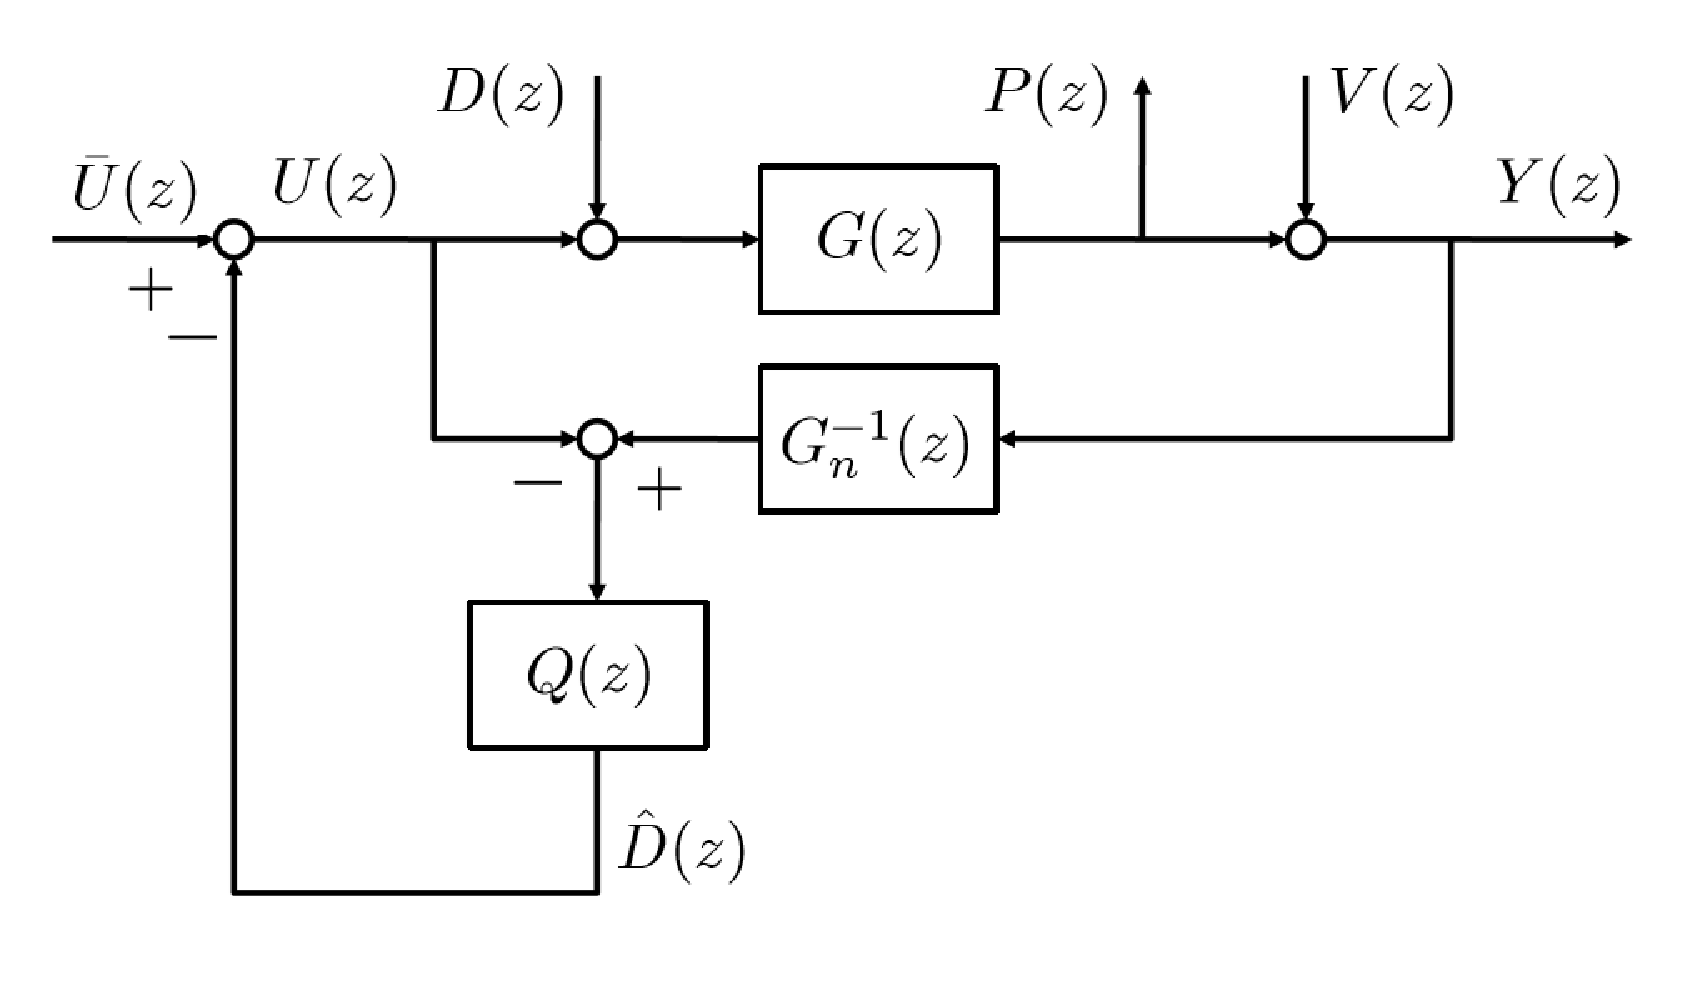
\includegraphics[width=0.5\textwidth]{Disturbance_Observer_DO}\\
    \end{figure}

    Concerns when choosing $Q(z)$:
    \begin{enumerate}
    \item[4.] \textbf{Realizability:}
    Choose $Q(z)$ so that $\hat{D}(z) = Q(z) [ G_n^{-1}(z) Y(z) - U(z)]$ is realizable
    \pause
    \newline

    $\Rightarrow$ Choose $Q(z)$ realizable so that $\displaystyle\frac{Q(z)}{G_n(z)}$ is also realizable
    \pause
    \newline

    This is a constraint on the relative degree of $Q(z)$

    \end{enumerate}
\end{frame} 